\subsection{Simulation test}\label{chapter_SimulationTest}

This chapter is about testing the Matlab/Simulink state space controller with the Matlab/Simulink process. Therefore the same control sequence of the remote input is used for the PID controller and the state space controller. A random sensor noise is enabled during the whole simulation time.

This sequence is:
\begin{enumerate}
\item{Start of simulation}
\item{At 2 seconds a \textit{phi} step to -0.35 rad (~-20 degree)}
\item{At 4 seconds a \textit{theta} step to 0.35 rad (~20 degree)}
\item{At 6 seconds a \textit{rpsi} step to 0.75 rad/s (~43 degree/s)}
\item{Start of simulation}
\end{enumerate}
 
After running this sequence (duration 10 seconds), there are several scopes used to check the result. Figures \ref{fig:Motor_PID} to \ref{fig:rpsi_PID} are showing the result, using the PID controller, figures \ref{fig:Motor2_SS} to \ref{fig:rpsi_SS} those, using the developed state space controller.

\begin{figure}
	\centering
		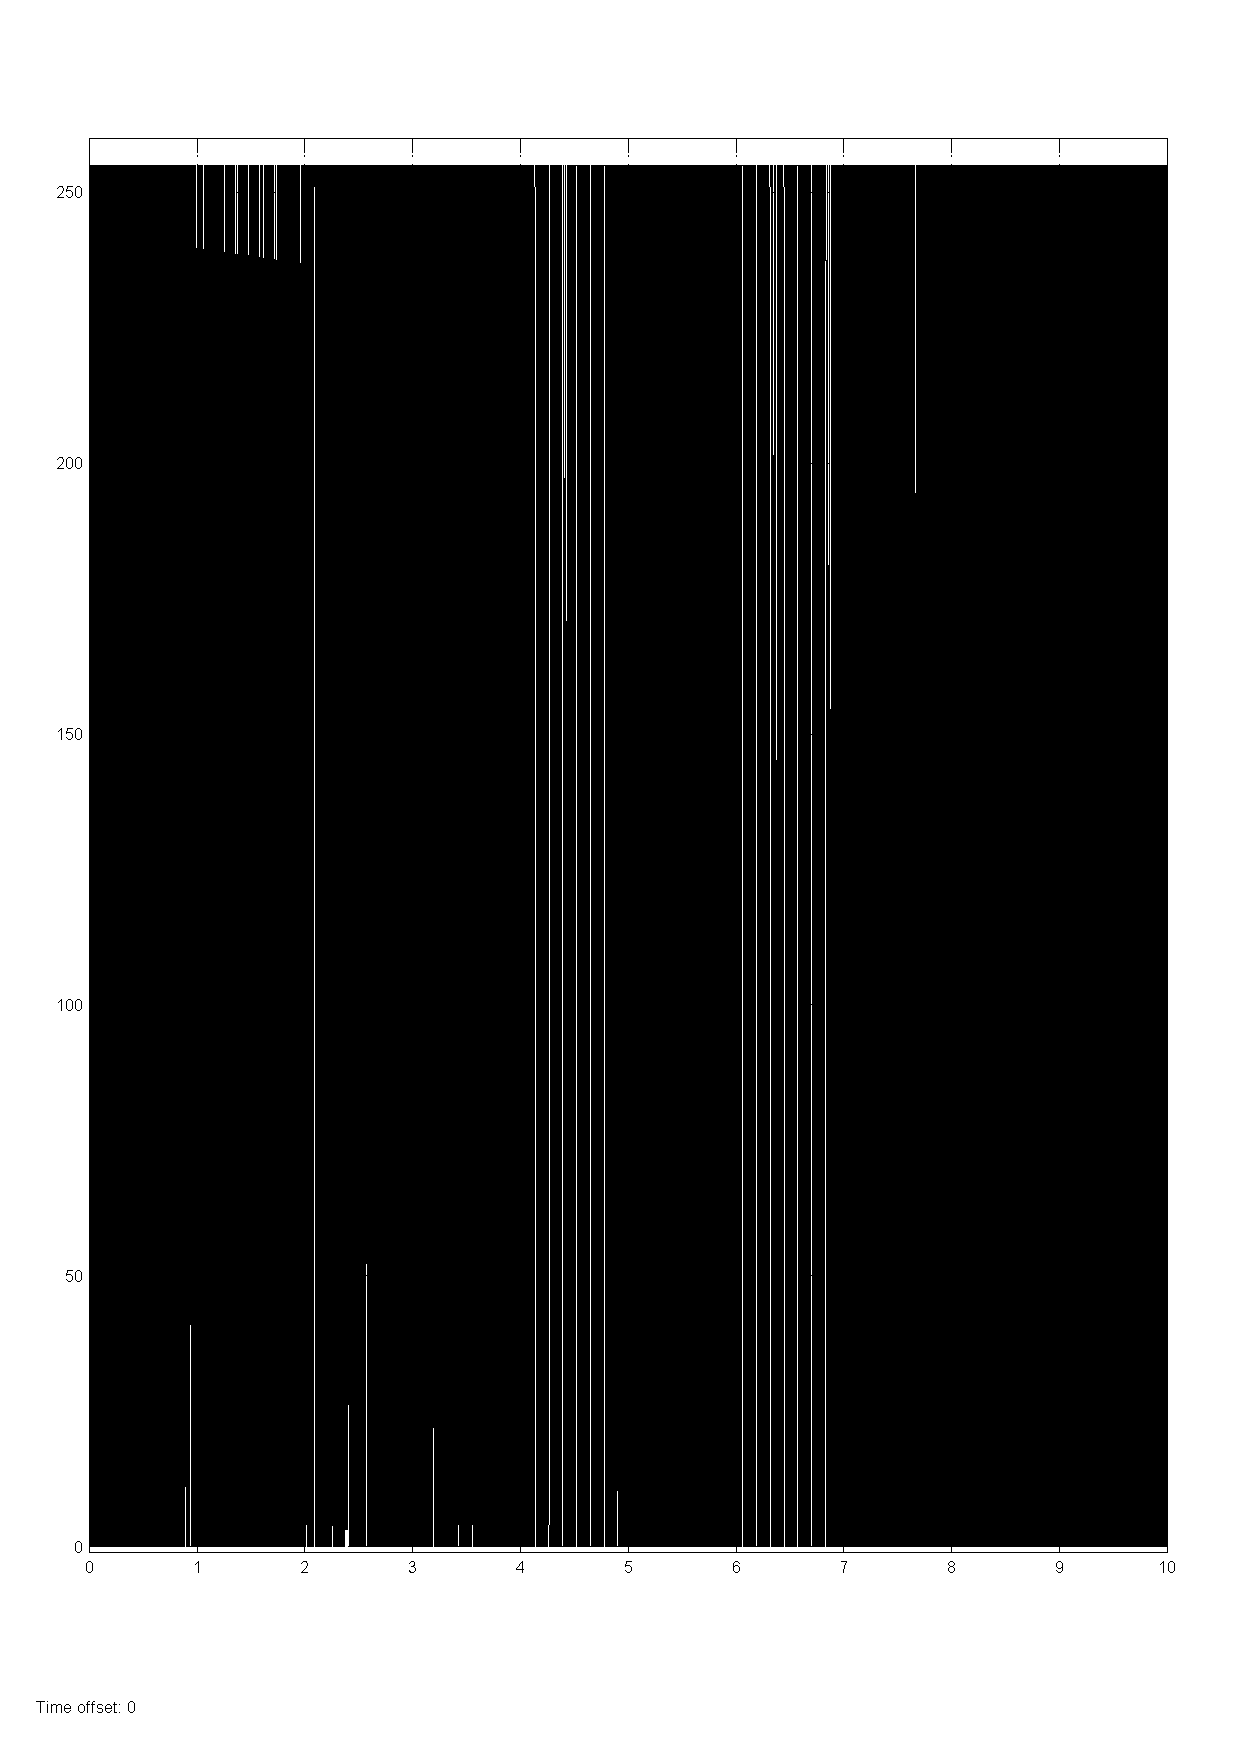
\includegraphics[width=0.3\textwidth]{03_Grafiken/Motor_PID.pdf}
	\caption{Set value for one motor using the PID controller}
	\label{fig:Motor_PID}
\end{figure}

Figure \ref{fig:Motor_PID} shows one of the four set values for the motor forces. That is no graphical error, but the PID controller pushes the actuating variables the whole time into the saturation of 255 and 0. Interestingly this strategy works, like the following figures are showing.

\begin{figure}
	\centering
		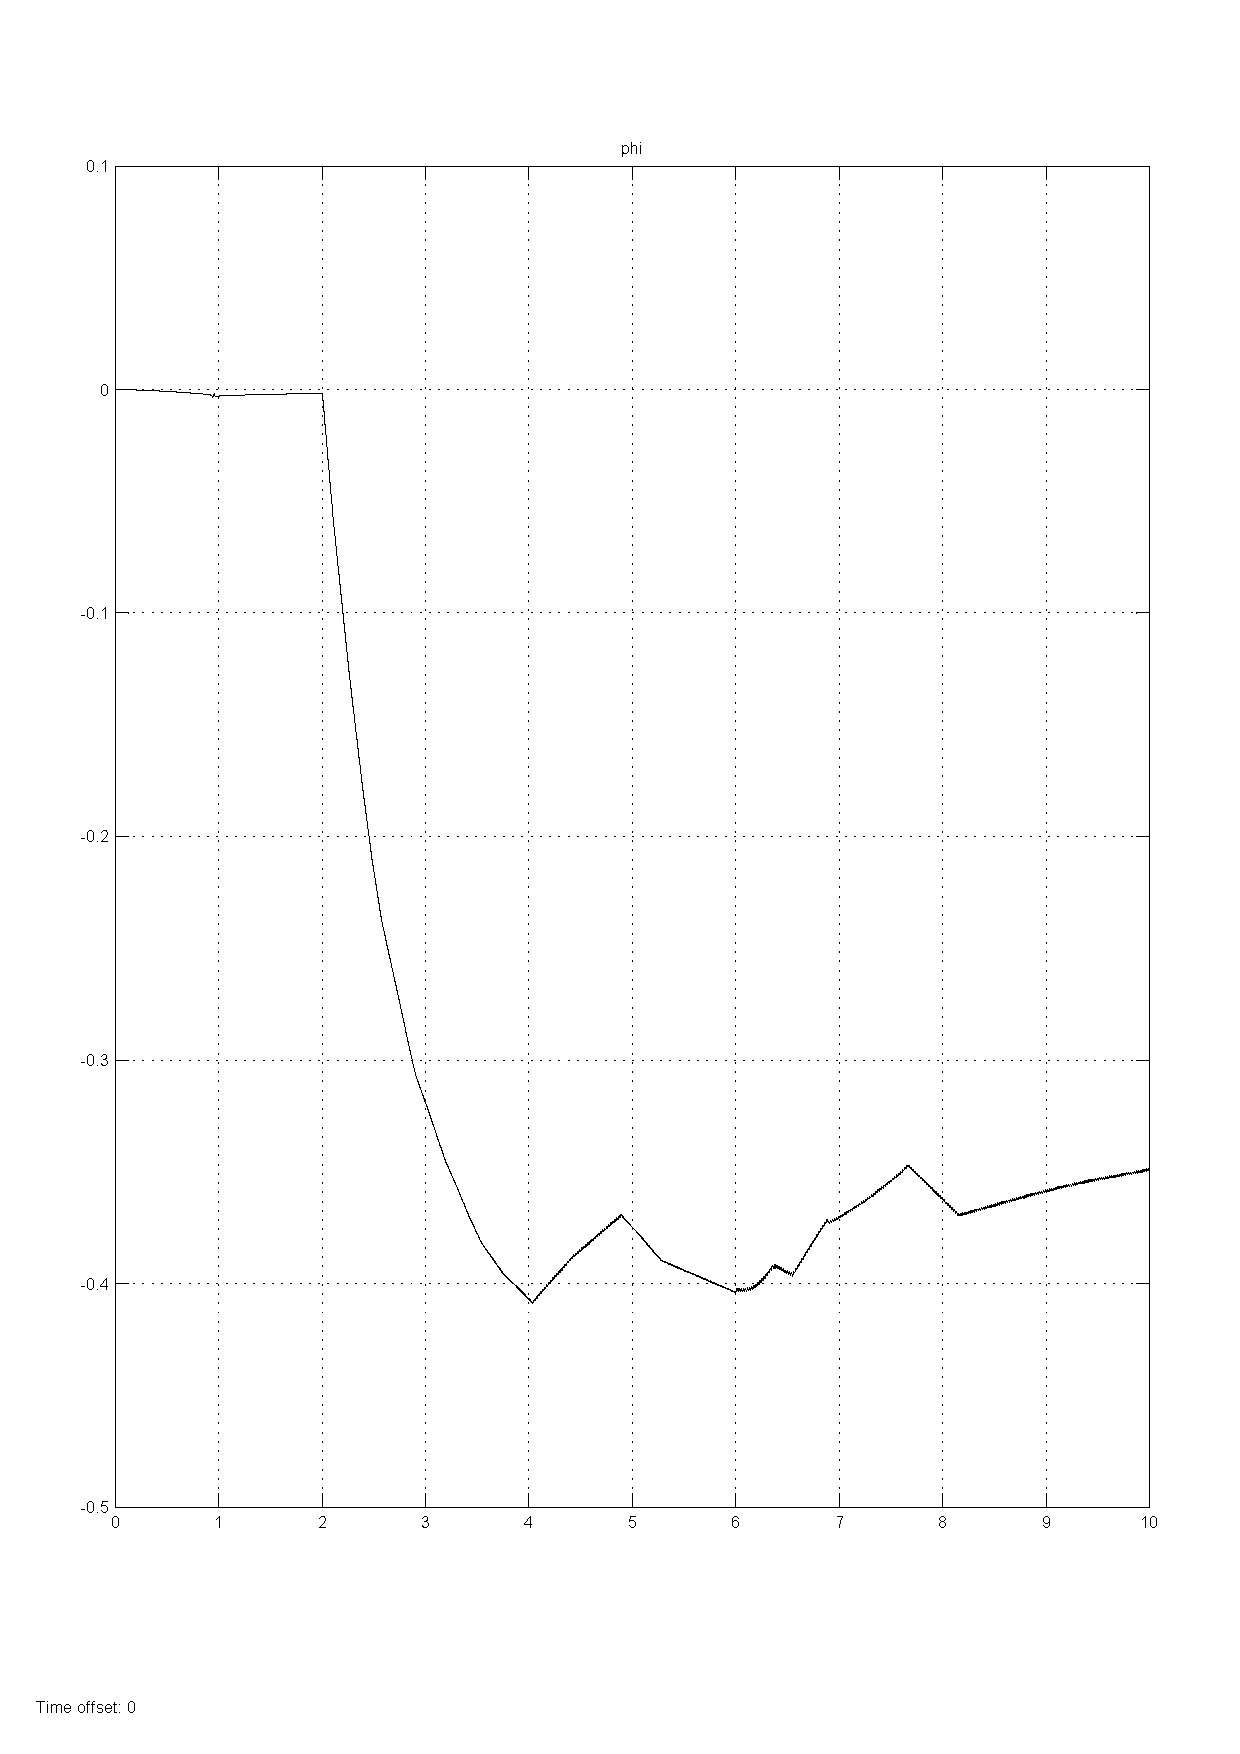
\includegraphics[width=0.8\textwidth]{03_Grafiken/phi_PID.pdf}
	\caption{Angle of phi using the PID controller}
	\label{fig:phi_PID}
\end{figure}

Figure \ref{fig:phi_PID} shows the angle of \textit{phi} after the whole sequence. The estimated angle is not hold stable. There are heavy influences at the time, the other two steps occur.

\begin{figure}
	\centering
		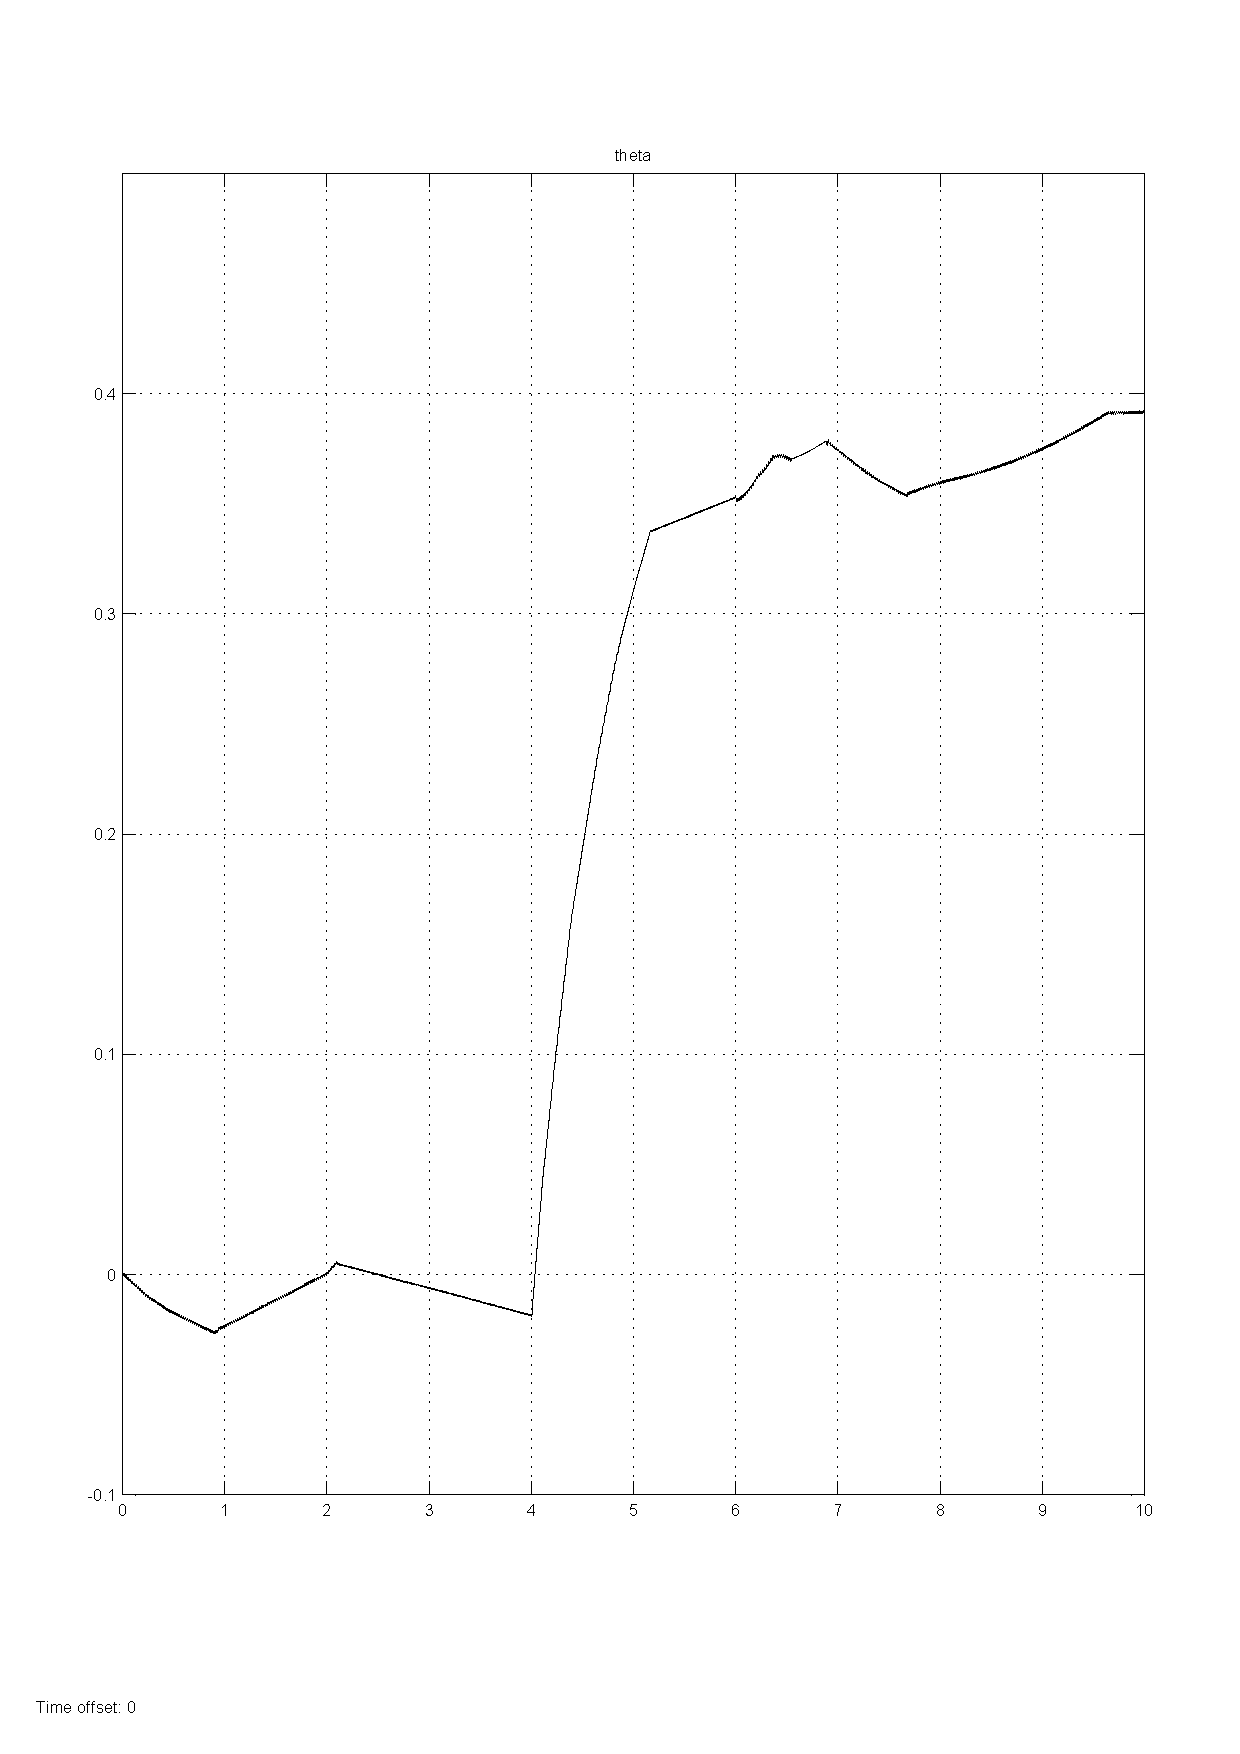
\includegraphics[width=0.8\textwidth]{03_Grafiken/theta_PID.pdf}
	\caption{Angle of theta using the PID controller}
	\label{fig:theta_PID}
\end{figure}

Figure \ref{fig:theta_PID} shows the angle of \textit{theta} after the whole sequence. It is the same as the angle of phi - the estimated angle is not hold stable and there are heavy influences at the time, the other two steps occur.

\begin{figure}
	\centering
		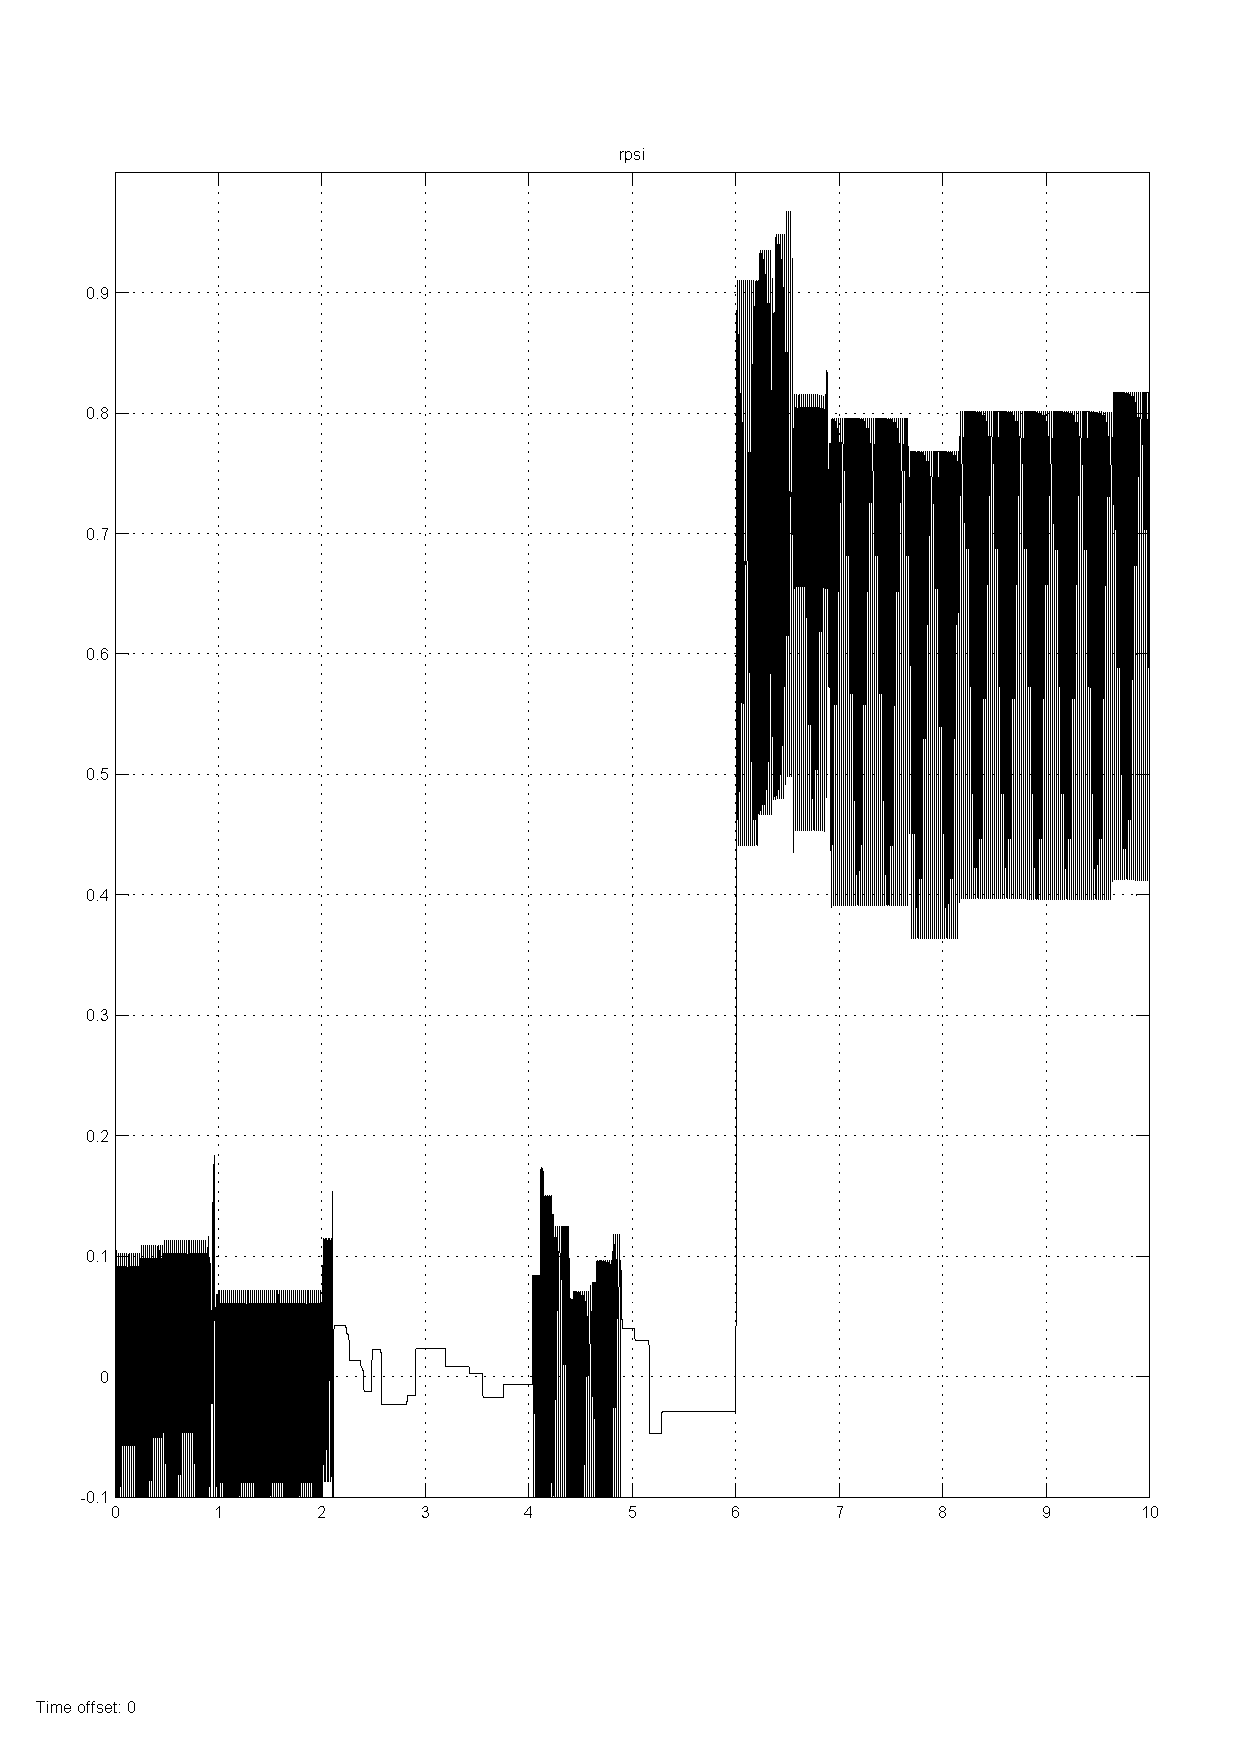
\includegraphics[width=0.8\textwidth]{03_Grafiken/rpsi_PID.pdf}
	\caption{Angular velocity of psi using the PID controller}
	\label{fig:rpsi_PID}
\end{figure}

Figure \ref{fig:rpsi_PID} shows the angular velocity of \textit{psi}, \textit{rpsi}, after the whole sequence. The rate is oscillating, but that is just the behavior of the simulation. In the real copter, the inertia of masses in movement prevents that.

The following figures are showing the same scopes, using the state space controller instead of the PID controller.

\begin{figure}
	\centering
		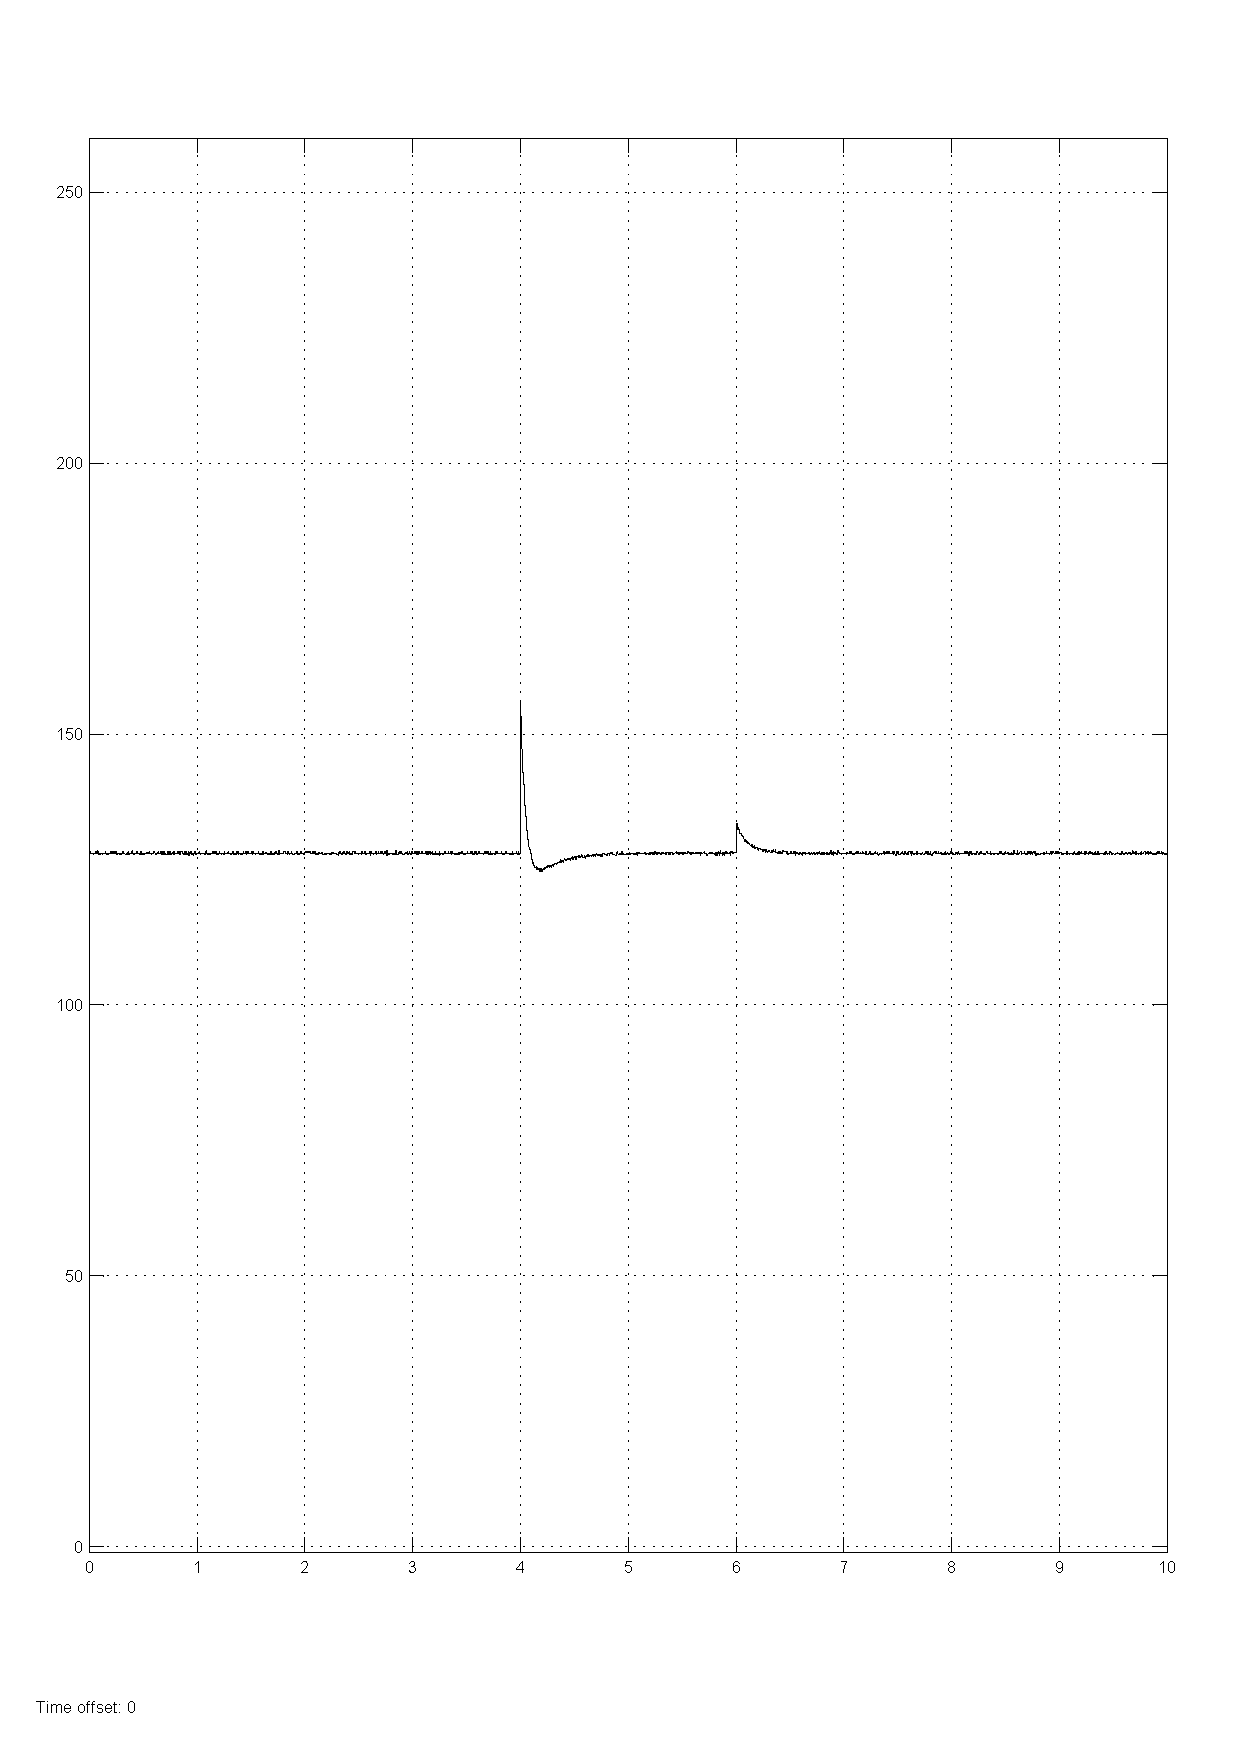
\includegraphics[width=0.8\textwidth]{03_Grafiken/Motor2_SS.pdf}
	\caption{Set value for one motor using the state space controller}
	\label{fig:Motor2_SS}
\end{figure}

In contrast to the PID controller, the state space controller does not push the actuating variables very high. There is just a little peak, at the moment the step occurs (Figure \ref{fig:Motor2_SS}).

\begin{figure}
	\centering
		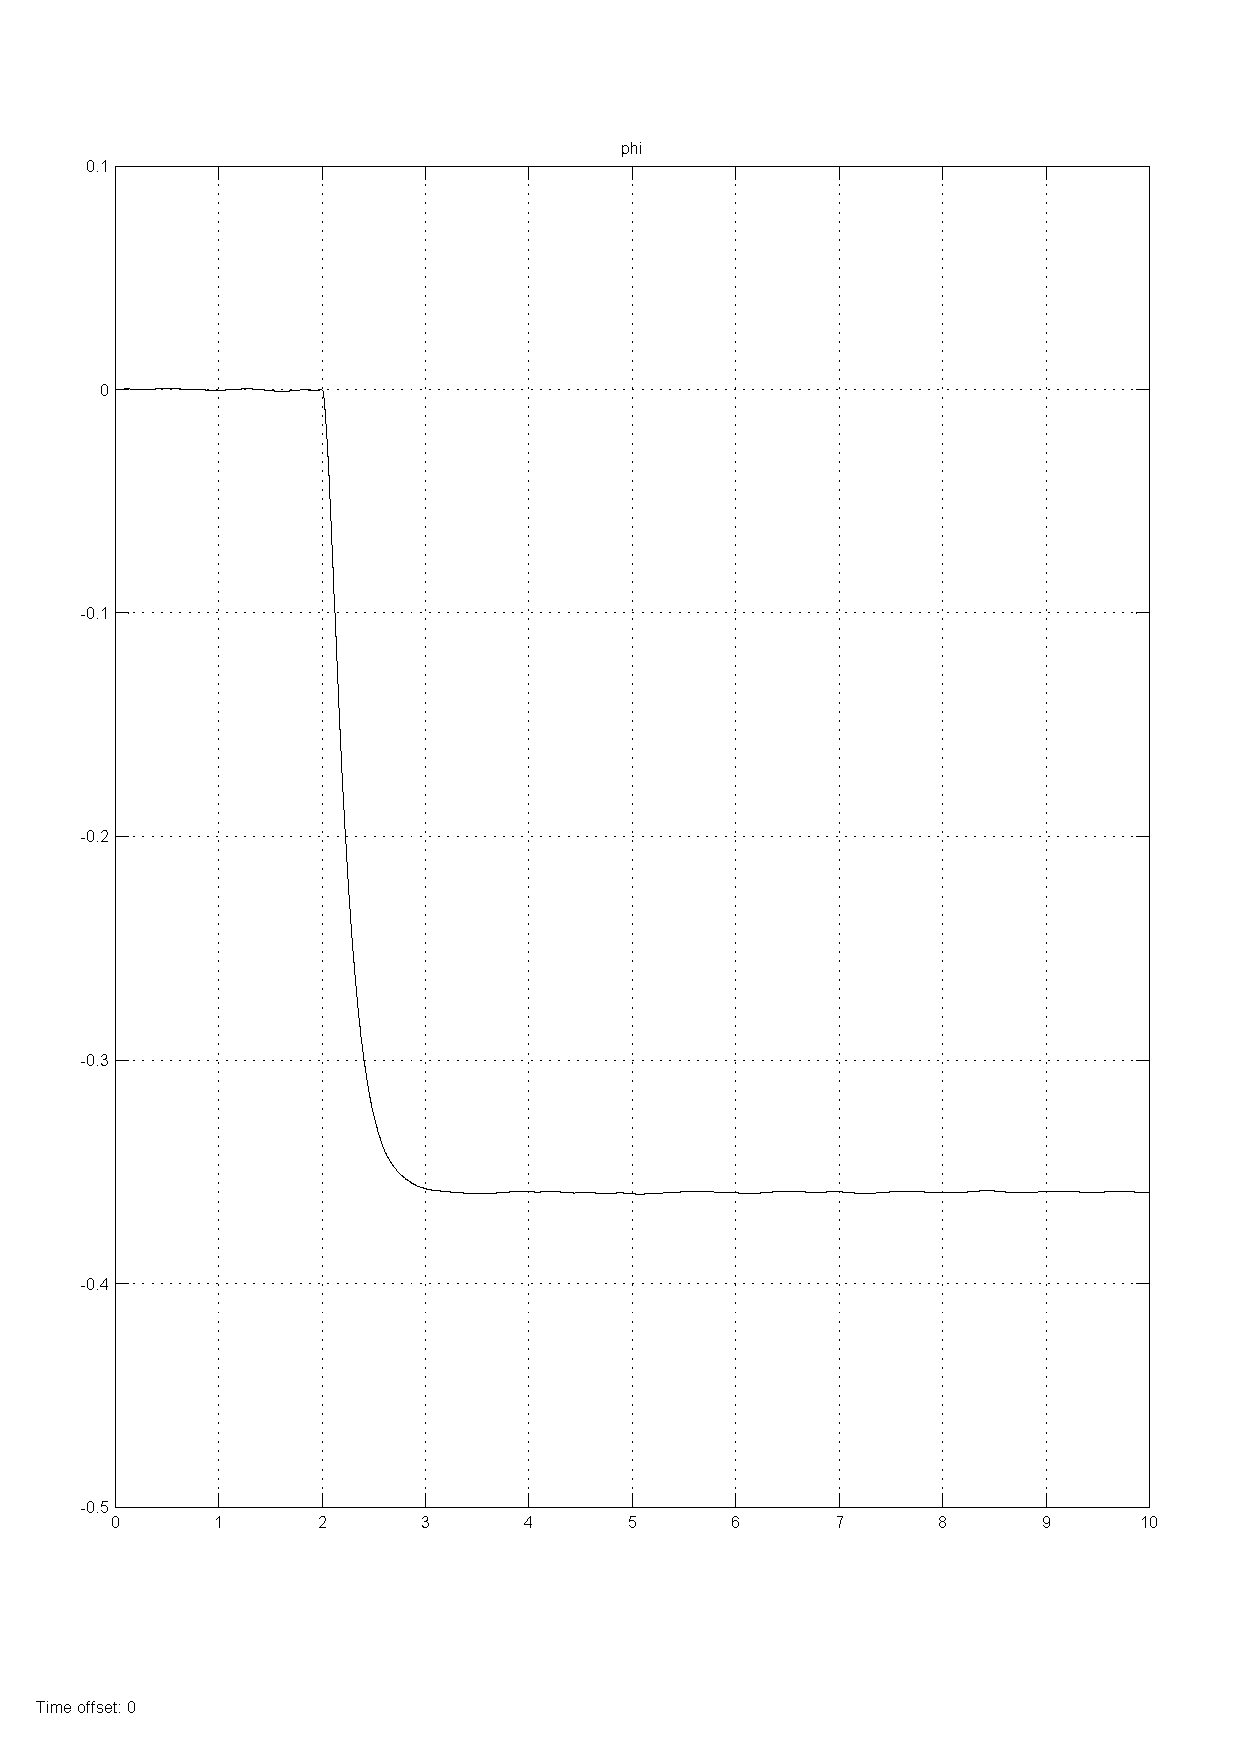
\includegraphics[width=0.8\textwidth]{03_Grafiken/phi_SS.pdf}
	\caption{Angle of phi using the state space controller}
	\label{fig:phi_SS}
\end{figure}

Figure \ref{fig:phi_SS} shows the angle of phi during the simulation. The estimated angle of -0.35 rad is reached within 0.5 seconds and is kept very accurate. Furthermore there is no influence of the other two steps at second four and second six.

\begin{figure}
	\centering
		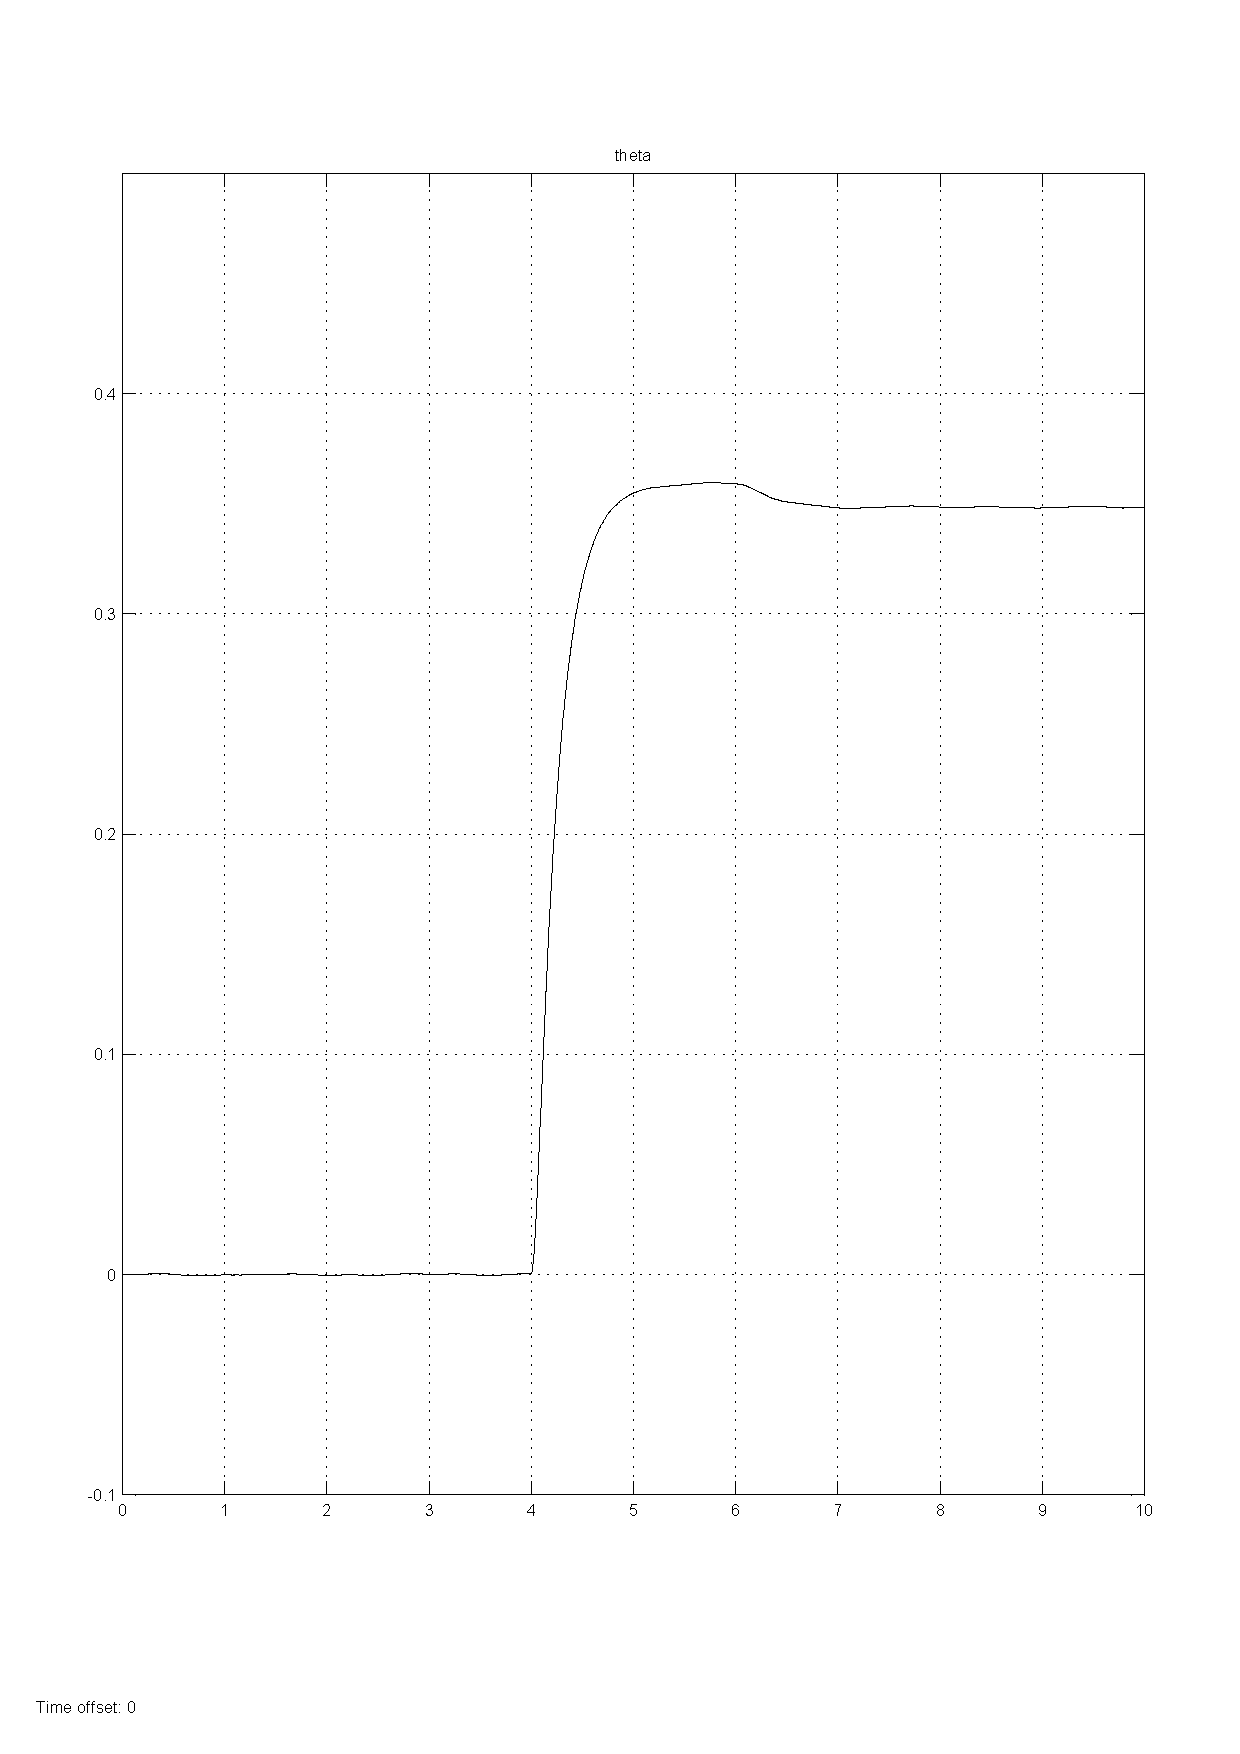
\includegraphics[width=0.8\textwidth]{03_Grafiken/theta_SS.pdf}
	\caption{Angle of theta using the state space controller}
	\label{fig:theta_SS}
\end{figure}

Figure \ref{fig:theta_SS} shows the angle of theta during the simulation. Like the angle of phi, the estimated angle of 0.35 rad is reached within 0.5 seconds. The step to the rate of psi at second six reduces the angle about approximately 0.015 rad, which is not even one degree and therefore insignificant small.

\begin{figure}
	\centering
		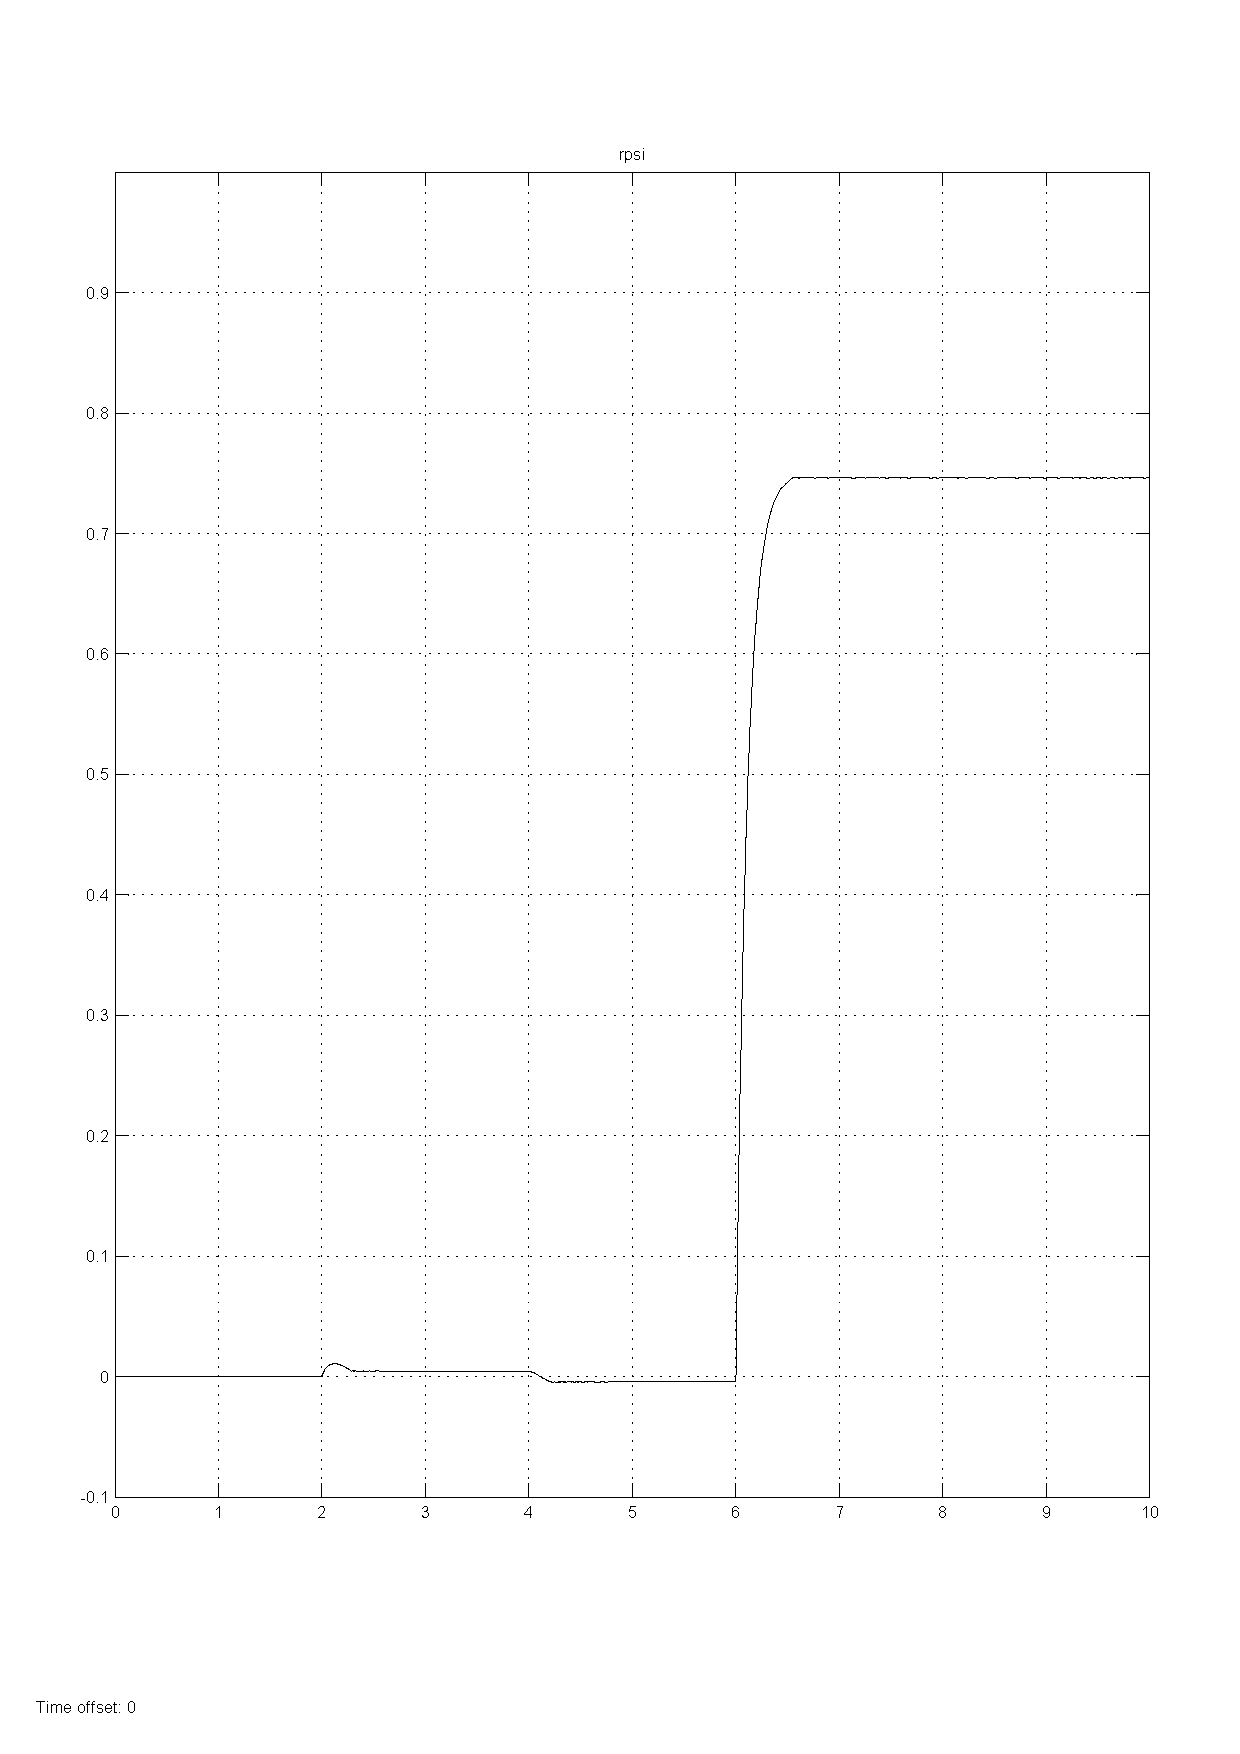
\includegraphics[width=0.8\textwidth]{03_Grafiken/rpsi_SS.pdf}
	\caption{Angular velocity of psi using the state space controller}
	\label{fig:rpsi_SS}
\end{figure}

Figure \ref{fig:rpsi_SS} shows the very fast and accurate behavior of the rate of psi. The rate is reached very fast within less than half a second.


All in all, the simulation of the developed state space controller went well, and the next step, the HIL tests, can be performed.